% Created 2024-10-27 Sun 04:11
% Intended LaTeX compiler: pdflatex
\documentclass[11pt]{article}
\usepackage[utf8]{inputenc}
\usepackage[T1]{fontenc}
\usepackage{graphicx}
\usepackage{longtable}
\usepackage{wrapfig}
\usepackage{rotating}
\usepackage[normalem]{ulem}
\usepackage{amsmath}
\usepackage{amssymb}
\usepackage{capt-of}
\usepackage{hyperref}
\usepackage{enumitem}
\usepackage{breqn}
\author{Charles Gannon}
\date{\today}
\title{Astro 204 Problem Set 4}
\hypersetup{
 pdfauthor={Charles Gannon},
 pdftitle={Astro 204 Problem Set 4},
 pdfkeywords={},
 pdfsubject={},
 pdfcreator={Emacs 29.4 (Org mode 9.8)}, 
 pdflang={English}}
\begin{document}

\maketitle
\tableofcontents

\section{Collapse and outflow}
\label{sec:orga7e0318}
The force on a patch of mass (\(dm\)) in the cloud from gravity is
\begin{equation}
 F_G = \frac{G M dm}{r^{2}},
\end{equation}
where r is the radial distance of the patch from the center of cloud, and M is the mass enclosed in radius r.
If the cloud was not pressure supported the radial acceleration would be
\begin{equation}\label{eq:ag}
 \ddot{r} = -\frac{G M}{r^{2}}.
\end{equation}
For a quick estimate of the time for the cloud to collapse, we can approximate the acceleration \(\ddot{r}\)  as constant.
Under this assumption, we can derive a relation for the \(t_{dyn}\) in terms of the initial radius of the patch \(r_{0}\)
\begin{equation}
 r_{0} = \frac{1}{2} \frac{G M}{r_{0}^{2}} t_{dyn}^{2},
\end{equation}
which solving for \(t_{dyn}\) gives
\begin{equation}
 t_{dyn} = \sqrt{\frac{2 r_{0}^{3}}{GM}}.
\end{equation}
If no shells cross during spherical collapse, the mass enclosed within a collapsing spherical shell (\(M\)) will remain constant.
Therefore, we can do better and solve \ref{eq:ag} exactly without assuming a density profile.
Assuming eq. \ref{eq:ag} has a solution of the form \(r = a (t - t_{0})^{n}\), then the equation becomes
\begin{equation}
 a n (n - 1) (t - t_{0})^{n-2} = \frac{GM}{a^{2} (t - t_{0})^{2n}},
\end{equation}
which to be valid forces \(n = 2/3\).
Solving for a yields
\begin{equation}
 a = -\left( \frac{9}{2} G M \right)^{1/3}.
\end{equation}
By plugging into our initial guess for the solution, we can again we can derive a relation for the dynamical time in terms of the initial radius
\begin{equation}
  t_{dyn} = \frac{1}{3}\sqrt{\frac{2 r_{0}^{3}}{G M}}.
\end{equation}
This solution doesn't have v(t=0)=0 !
Note that the exact solution and estimate only differ by a factor of \(1/3\)
The time for sound to reach the center of the cloud if it starts at \(r = r_{0}\) (sound crossing time, \(t_{c}\)) and the speed of sound in the gas \(c_s\) is constant is
\begin{equation}
 t_{c} = \frac{r_{0}}{c_{s}}
\end{equation}
A gas under hydrostatic equilibrium obeys the equation
\begin{equation}\label{eq:hydroeq}
 \frac{1}{\rho} \frac{d P}{d r} = \frac{G M}{r^{2}}
\end{equation}
where P is the pressure of the gas and \(\rho\) is it's density.
The right hand of eq. \ref{eq:hydroeq} can be re-written in terms of \(t_{dyn}\)
\begin{equation}\label{eq:left}
 \frac{G M}{r^{2}} \sim -\frac{r}{t_{dyn}^{2}},
\end{equation}
where I have dropped all constant coefficients.
Likewise, the left hand of the equation can be written in terms of the crossing time.
Using the ideal gas law
\begin{equation}
 P = c_{s}^{2} \rho,
\end{equation}
we can rewrite the pressure of the gas in terms of the density.
In order to proceed, I assume the density can be written as a power law in terms of the radius
\begin{equation}
 \rho = b r^{-\gamma}.
\end{equation}
Under these assumptions, the left hand of \ref{eq:hydroeq} becomes
\begin{equation}\label{eq:left}
 \frac{1}{\rho} \frac{d P}{dr} \sim -\frac{c_{s}^{2}}{r} = -\frac{r}{t_{c}^{2}},
\end{equation}
where I again have dropped all constant coefficients.
Putting everything back together gives
\begin{equation}
 t_{c} \sim t_{dyn}.
\end{equation}
For the cloud to collpase, the absolute value of the force of gravity acting on a patch must be greater than the absolute value of the force from the pressure
\begin{equation}
 \frac{dP}{dr} < \frac{G M \rho}{r^{2}}.
\end{equation}
Using our previously previous results this implies
\begin{equation}
  \frac{1}{t_{c}^{2}} < \frac{1}{t_{dyn}^{2}}
\end{equation}
which can be simplified to
\begin{equation}
 t_{dyn} < t_{c}
\end{equation}
meaning if the dynamical time is less than the sound crossing time the cloud will collapse.
Likewise, for the cloud to fly appart
\begin{equation}
  \frac{1}{t_{c}^{2}} > \frac{1}{t_{dyn}^{2}}
\end{equation}
which rewriting in terms of the escape velocity
\begin{equation}
 v_{esc} = \sqrt{\frac{2 G M}{r}} \sim \frac{r}{t_{dyn}}
\end{equation}
and speed of sound in the cloud gives the condition
\begin{equation}
 c_{s} > v_{esc}.
\end{equation}
Therefore,  for the cloud to fly apart the speed of sound in the medium must be larger than the escape velocity.
\section{Parker Winds}
\label{sec:org55482c9}
\begin{enumerate}[label=\alph*)]
 \item
  Bernoulli's constant along a stream line is
  \begin{equation}
   B = \frac{1}{2} v^{2} + h + \phi
  \end{equation}.
  For a parker wind the potential is gravitational
  \begin{equation}
   \phi = - \frac{GM}{r}
  \end{equation}

  The enthalpy of a system is
  \begin{equation}
   dH = dU + pdV,
  \end{equation}
  which can be rewritten in term of enthalpy per mass
  \begin{equation}
   dh = \frac{1}{\rho} dP + T ds,
  \end{equation}
  or for constant entropy
  \begin{equation}
   h = \int_{S} \frac{dP}{\rho}
  \end{equation}.
  For our equation of state we have
  \begin{equation}
   P = c_s^2 \rho,
  \end{equation}
  which when gives mean our system has entahlpy given by
  \begin{equation}
   h = c_s^2 ln \rho + C.
  \end{equation}
  Plugging everything in,
  \begin{equation}
    \frac{1}{2} v^2 + ln \rho - \frac{G M}{r} = \text{const}
  \end{equation}
  to further simplify we can use the mass loss rate of our system
  \begin{equation}
   \dot{M} = 4 \pi r^2 \rho v
  \end{equation}
  where our mass loss rate, $\dot{M}$ is constant to maintain a steady state solution.
  Solving for $\rho$ and plugging into our expression for the Bernoulli constant gives
  \begin{equation}
    \frac{1}{2} v^2 - c_s^2(\ln r - 2 \ln v)  - \frac{G M}{r} = \text{const}
  \end{equation}
  Rearanging and substituting $r_s = \frac{GM}{2c_s^2}$ gives
  \begin{equation}
   \ln v - \frac{1}{2} \frac{v^2}{c_s^2} = - 2 \ln r - 2 \frac{rs}{r} + \text{const},
  \end{equation}
  which taking the exponent gives
  \begin{equation}
   v e^{-v^2/(2c_s^2)} = Cr^{-2}e^{-2r_s/r}.
  \end{equation}
  By imposing  $v(r_s) = c$ we get
  \begin{equation}
   c_s e^{-1/2} = C r_s^{-2}e^{-2},
  \end{equation}
  which when solved for C gives
  \begin{equation}
   C = c_s r_s^2 e^{3/2}.
  \end{equation}
  Putting everything together we have
  \begin{equation}
   v e^{-v^2/(2c_s^2)} = c_s \left( \frac{r_s}{r} \right)^2 e^{(3/2) - 2r_s/r }.
  \end{equation}
 \item
  The mass equation is
  \begin{equation}
   \frac{\partial \rho}{\partial t} + \vec{\nabla} \cdot (\rho \vec{v}) = 0
  \end{equation}
  Since a parker wind is in steady state, $\frac{\partial \rho}{\partial t} = 0$.
  Furthermore, the velocity of a park wind only radial compont so $\vec{\nabla} \cdot (\rho \vec{v}) = \frac{1}{r^2} (r^2 \rho v)$.
  Therefore the mass equation becomes
  \begin{equation}
    0 = \frac{1}{r^2} (r^2 \rho v) = r^2 v_r \frac{\partial \rho}{\partial r} + 2 r \rho + r^2 \rho \frac{\partial v}{\partial r}
  \end{equation}
  The momentum equation is
  \begin{equation}
   \rho \frac{d \vec{v}}{d t} = - \vec{\nabla} P + \rho \frac{GM}{r^2}.
  \end{equation}
  We know $P = c_s^2 \rho$, aditionlly from the chain rule $\frac{d \vec{v}}{dt} = \vec{v} \cdot \frac{\partial v}{\partial r}$.
  Therefore the momentum equation becomes
  \begin{equation}
   \rho v \frac{\partial v}{\partial r} = -c_s^2 \frac{\partial \rho}{\partial r} - \rho \frac{GM}{r^2} .
  \end{equation}
  Plugging in the mass equation we get
  \begin{equation}
   \rho v \frac{\partial v}{\partial r} = -c_s^2 \rho (-\frac{2}{r} - \frac{1}{v}\frac{\partial v}{\partial r} )  - \rho \frac{GM}{r^2} .
  \end{equation}
  After some simplification and noting that the partial derivatives are equivalent to the total derivative the equation becomes
  \begin{equation}
   \frac{1}{v} \frac{d v}{dr} (v^2 - c_s^2) = \frac{2 c_s^2}{r} - \frac{G M}{r^2}
  \end{equation}
 \item
  See the fig \ref{fig:problem2c} for plots, and problem2c.py for code.

 \item

  The mass change rate for parker wind is
  \begin{equation}
   \dot{M} = 4 \pi r^2 \rho v,
  \end{equation}
  so
  \begin{equation}
    \rho = \frac{\dot{M}}{4 \pi r^2 v} = \rho_s \left ( \frac{r_s}{r} \right )^2 \frac{c_0}{v}.
  \end{equation}
  We may rewrite and get an expression for velocity
  \begin{equation}
    v = c_s \left ( \frac{r_s}{r} \right )^2 \frac{\rho_s}{\rho}
  \end{equation}
  which we can plug into our trancendental velocity equation.
  After some simplifying I arrive at
  \begin{equation}
    \frac{\rho}{\rho_0} e^{\frac{1}{2} \left( \frac{r_0^2 \rho_0 v_0}{r^2 \rho c_S} \right)^2} = e^{\frac{-2 r_s}{r_0}(1-r_0/r) + \frac{1}{2}\left(  v_0 / c_s\right)^2}
  \end{equation}
  which is the same as the hydrostatic solution if $v_0 << c_S$ and $r_0^2 \rho_0 v_0 < r^2 \rho c_s$.
 \item
  The outflow timescale is $t_s \sim r_s/c_s$, a quick way of seeing this is that our equation have one length scale: $r_s$ and one velocity scale $v_s$.
  Using dimensional analysis, we can combine these scales to get a time scale by dividing them.
  Plugging everything in with $M_e = 10^{24}$ kg, and the speed of sound for hydrogen at $10000$ K, $c_S \approx 2.9 \cdot 10^3$ m/s I get 2.16 hours (appologies for the SI units).
  The actual value was 4 hours so this is very close!


\end{enumerate}

\begin{figure}[htbp]
\centering
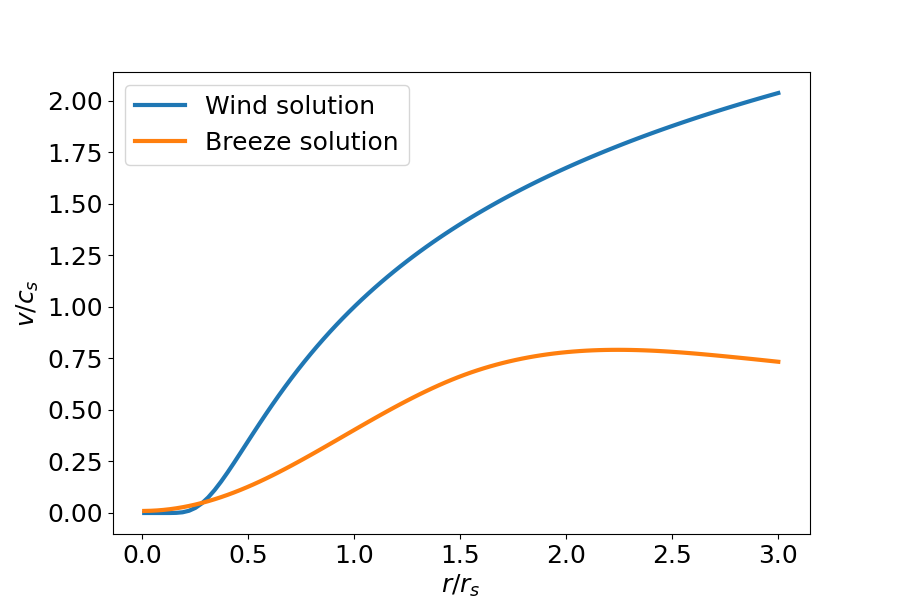
\includegraphics[width=.9\linewidth]{../plots/windbreeze.png}
\caption{\label{fig:problem2c}The numerical solutions for part (c).}
\end{figure}
\end{document}
